\subsection{Reference model for Open Source Software Processes Discovery}
Jensen \& Scacchi in \cite{citeulike:5043664} take a somewhat different approach from the previously discussed research efforts. The authors are follow a top-down approach and do not try to build a software process model from available process artifacts. Instead, they try to develop a software process \textit{reference model} by iteratively refining mapping between observed artifacts and the model entities. 

The proposed software process \textit{reference model} is a layer which provides a mapping from the underlying recognized software process artifacts into a higher level software-process meta-model by Mi \& Sacchi \cite{citeulike:5128872}. The iterative revision of the reference model vocabulary of mapped terms (Figure \ref{fig:refterm}) is performed through case studies. During such a study, the observed process artifacts such as SCM logs, defect reports and others are queried with terms from the reference model pulling correlated artifacts which are revised and curated by the process expert and lead to the further revisions of the terms taxonomy on the next iteration.

\begin{figure}[tbp]
   \centering
   \includegraphics[height=40mm]{refterm.eps}
   \caption{Example of the reference model mapping from \cite{citeulike:5043664}.}
   \label{fig:refterm}
\end{figure}

In the relation to my research, I am envisioning the application of such iterative ``meta-model driven approach'' for characterization of the discovered recurrent patterns with unknown generative phenomena. The creation of the low-level recurrent patterns taxonomy through successive mapping into the meta-model assures from a ``nonsense patterns'' discovery.